\section{EAR (Estrutura Analítica de Riscos)} % (fold)
\label{sec:ear_estrutura_analítica_de_riscos_}

	Para auxiliar na identificação das fontes riscos durante a execução do projeto, foi elaborado uma estrutura analítica de riscos (EAR), que pode ser visualizada na Figura \ref{img:ear}.

	\begin{figure}[H]
		\centering
		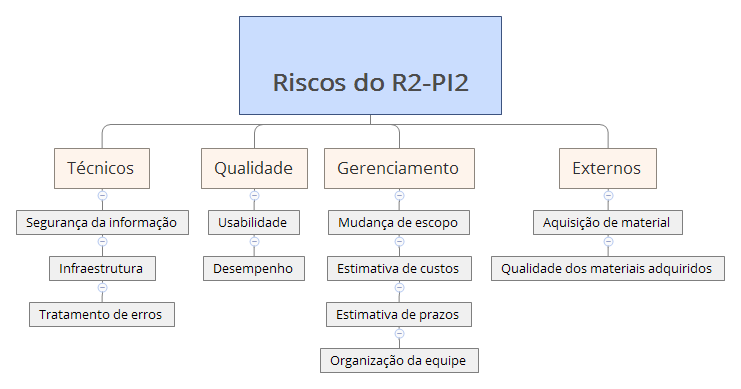
\includegraphics[scale=0.55]{figuras/ear.png}
		\caption{Estrutura analítica de riscos.}
		\label{img:ear}
	\end{figure}

	Os principais tipos de riscos identificados no projeto são:

	\begin{itemize}
		\item \textbf{Técnicos}: 
			
			Riscos relacionados às tecnologias do sistema.

		\item \textbf{Qualidade}: 
			
			Riscos relacionados à qualidade final do sistema.

		\item \textbf{Externos}:

			Riscos externos à equipe de desenvolvimento.

		\item \textbf{Gerenciamento de Projetos}:

			Riscos relacionados às questões de gerência do projeto e organização interna.
	
	\end{itemize}
% section ear_estrutura_analítica_de_riscos_ (end)

\section{Identificação dos Riscos} % (fold)
\label{sec:identificação_dos_riscos}
	
	Foi utilizada a técnica de \textit{Brainstorming} e reuniões em equipe para a identificação dos riscos do projeto, de modo que todas as áreas fossem analisadas e que os riscos principais do projeto fossem identificados a fim de dar uma nota para os aspectos “probabilidade” e “impacto” para avaliar a necessidade de um plano de resposta. A tabela abaixo mostra os riscos identificados e as suas atribuições de nota.

	Por motivos de espaço, a tabela dos riscos identificados foi quebrada em 3 (três) imagens, apresentadas em \ref{img:risco1}, \ref{img:risco2} e \ref{img:risco3}.

	\begin{figure}[H]
		\centering
		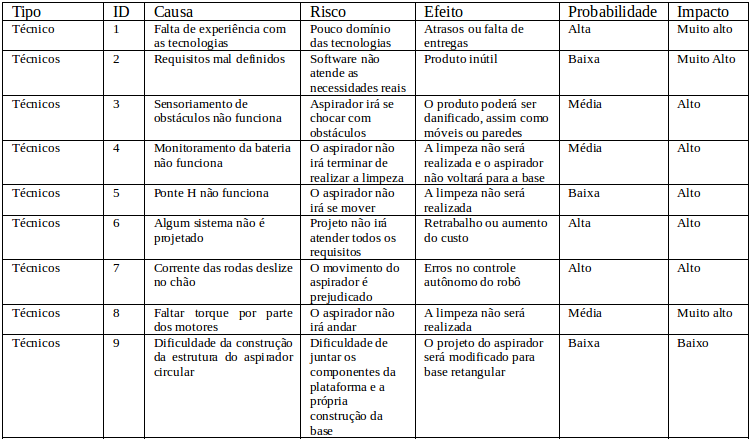
\includegraphics[scale=0.6]{figuras/riscos1.png}
		\caption{Riscos identificados 1.}
		\label{img:risco1}
	\end{figure}

	\begin{figure}[H]
		\centering
		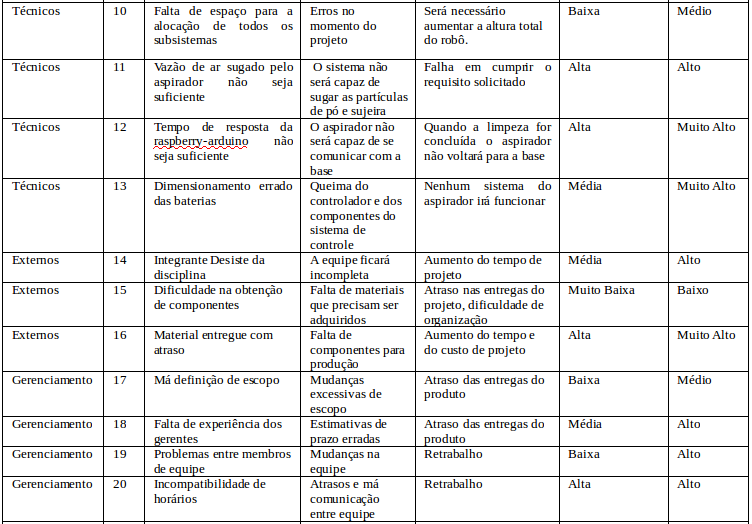
\includegraphics[scale=0.6]{figuras/riscos2.png}
		\caption{Riscos identificados 2.}
		\label{img:risco2}
	\end{figure}

	\begin{figure}[H]
		\centering
		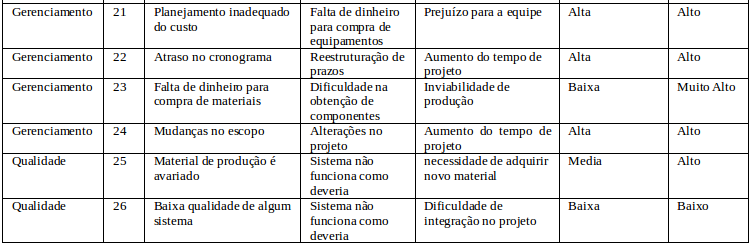
\includegraphics[scale=0.6]{figuras/riscos3.png}
		\caption{Riscos identificados 3.}
		\label{img:risco3}
	\end{figure}
	
% section identificação_dos_riscos (end)

\section{Análise Qualitativa dos Riscos} % (fold)
\label{sec:análise_qualitativa_dos_riscos}

	Para realizar a priorização dos riscos, é necessário uma análise qualitativa dos riscos, avaliando a probabilidade de ocorrência e o impacto de cada risco que será descrito A tabela a seguir mostra o resultado dessa análise.

	\begin{figure}[H]
		\centering
		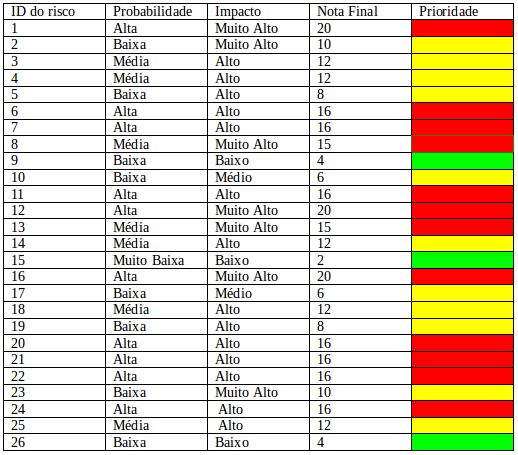
\includegraphics[scale=0.8]{figuras/riscosQualitativo.png}
		\caption{Qualificação dos riscos.}
		\label{img:ear}
	\end{figure}
% section análise_qualitativa_dos_riscos (end)

\section{Controle e mudança de riscos} % (fold)
\label{sec:controle_e_mudança_de_riscos}

	Com relação ao controle de riscos, para o projeto do R2-PI2, foram decididas as seguintes ações: 
	\begin{itemize}
		\item Os riscos serão controlados nas reuniões semanais
		\item Caso um novo risco seja identificado ou mesmo ocorrido, os gerentes devem reavaliar o risco qualitativamente e se ele atingir uma pontuação de 0,3 ou mais na matriz de impacto x probabilidade, deve-se planejar uma resposta para ele.
		\item Caso o item anterior ocorra, este plano de riscos deve ser atualizado.
	\end{itemize}
% section controle_e_mudança_de_riscos (end)

\section{Plano de Resposta aos Riscos} % (fold)
\label{sec:plano_de_resposta_aos_riscos}

	Para os riscos da zona amarela ( cuja estratégia não será aceitação)e os da zona vermelha, foram identificadas as seguintes ações de resposta:

	\begin{table}[H]
\centering
\caption{Resposta aos riscos.}
\label{tab:resposta}
\begin{tabular}{|c|c|c|c|}

\hline

\textbf{Risco}                                                                                           & \textbf{Ação}                                                                                                                                                                                & \textbf{Estratégia} & \textbf{Responsável}                                                  \\ \hline
\begin{tabular}[c]{@{}l@{}}Pouco domínio \\ das tecnologias\end{tabular}                                 & \begin{tabular}[c]{@{}l@{}}Treinamento com membros \\ mais experientes\end{tabular}                                                                                                          & Mitigar             & Desenvolvedores                                                       \\ \hline
\begin{tabular}[c]{@{}l@{}}Algum sistema \\ não é projetado\end{tabular}                                 & \begin{tabular}[c]{@{}l@{}}Alocar outros integrantes \\ para realização da tarefa\end{tabular}                                                                                               & Mitigar             & Desenvolvedores                                                       \\ \hline
\begin{tabular}[c]{@{}l@{}}Corrente das rodas \\ deslize no chão\end{tabular}                            & \begin{tabular}[c]{@{}l@{}}Será dimensionado uma \\ esteira emborrachada para \\ aumentar o atrito com o solo\end{tabular}                                                                   & Mitigar             & Desenvolvedores                                                       \\ \hline
\begin{tabular}[c]{@{}l@{}}Faltar torque por\\ parte dos motores\end{tabular}                            & \begin{tabular}[c]{@{}l@{}}Aumentar a tensão de \\ funcionamento do motor \\ ou a substituição do mesmo\end{tabular}                                                                         & Mitigar             & Desenvolvedores                                                       \\ \hline
\begin{tabular}[c]{@{}l@{}}Vazão de ar sugado \\ pelo aspirador não \\ seja suficiente\end{tabular}      & \begin{tabular}[c]{@{}l@{}}Aumentar a tensão sobre os\\  motores elétricos do cooler \\ ou aumentar o número de coolers \\ em paralelo, até que o problema \\ seja solucionado.\end{tabular} & Mitigar             & Desenvolvedores                                                       \\ \hline
\begin{tabular}[c]{@{}l@{}}Tempo de resposta \\ da raspberry-arduino \\ não seja suficiente\end{tabular} & \begin{tabular}[c]{@{}l@{}}Utilizar de tecnologias mais \\ velozes, ou com processamento \\ local.\end{tabular}                                                                              & Mitigar             & Desenvolvedores                                                       \\ \hline
\begin{tabular}[c]{@{}l@{}}Dimensionamento \\ errado das baterias\end{tabular}                           & \begin{tabular}[c]{@{}l@{}}Olhar especificações técnicas \\ de todos os componentes ou \\ trocar a bateria.\end{tabular}                                                                     & Mitigar             & Externos                                                              \\ \hline
\begin{tabular}[c]{@{}l@{}}Material entregue \\ com atraso\end{tabular}                                  & \begin{tabular}[c]{@{}l@{}}Antecipar o pedido dos \\ materiais.\end{tabular}                                                                                                                 & Mitigar             & Desenvolvedores                                                       \\ \hline
\begin{tabular}[c]{@{}l@{}}Má definição \\ de escopo\end{tabular}                                        & \begin{tabular}[c]{@{}l@{}}Redefinir escopo o mais \\ rápido possível.\end{tabular}                                                                                                          & Mitigar             & \begin{tabular}[c]{@{}l@{}}Gerentes e \\ desenvolvedores\end{tabular} \\ \hline
\begin{tabular}[c]{@{}l@{}}Incompatibilidade \\ de horários\end{tabular}                                 & \begin{tabular}[c]{@{}l@{}}Reuniões via Google Hangout \\ semanais em um horário \\ onde todos podem.\end{tabular}                                                                           & Mitigar             & Gerentes                                                              \\ \hline
\begin{tabular}[c]{@{}l@{}}Planejamento \\ inadequado do \\ custo\end{tabular}                           & Realizar novo planejamento.                                                                                                                                                                  & Mitigar             & Gerentes                                                              \\ \hline
Atraso no cronograma                                                                                     & \begin{tabular}[c]{@{}l@{}}Aumentar o esforço do tempo \\ de projeto restante.\end{tabular}                                                                                                  & Mitigar             & \begin{tabular}[c]{@{}l@{}}Gerentes e \\ desenvolvedores\end{tabular} \\ \hline
\begin{tabular}[c]{@{}l@{}}Falta de dinheiro \\ para compra de \\ materiais\end{tabular}                 & Buscar novas fontes de recurso.                                                                                                                                                              & Mitigar             & Desenvolvedores        \\ \hline                                              
\end{tabular}
\end{table}
% section plano_de_resposta_aos_riscos (end)
% section responsabilidade_dos_riscos_da_equipe_do_projeto (end)